\documentclass[12pt]{article}

\usepackage{sbc-template}
\usepackage{graphicx,url}
\usepackage[utf8]{inputenc}
\usepackage[brazil]{babel}
\usepackage{amsmath}
\usepackage{booktabs}
\usepackage{tabularx}
\usepackage{placeins}

\sloppy

\title{Mineração de Métricas DORA em Repositórios Open-Source:\\Um Estudo Empírico e Análise de Sensibilidade}

\author{Vinícius Simões\inst{1}, Maria Clara Gomes\inst{1}, Áulus H. Z. Pinto\inst{1}}

\address{Curso de Engenharia de Software -- Pontifícia Universidade Católica de Minas Gerais (PUC Minas)\\
  Belo Horizonte -- MG -- Brasil
  \email{\{vinisv2004, mariaclariagomes\}@gmail.com, aulus.pinto@sga.pucminas.br}
}

\begin{document} 

\maketitle
\begin{quote}
\textbf{Estado após integrar a main 4e05345 (21/10/2026).}
Os números e figuras recebidos para RQ05--RQ07 são preservados como material do grupo ainda não validado empiricamente. Não sustentam conclusões oficiais nem validação humana. A evidência exata e os comandos estão em \texttt{ENTREGA\_LAB03S03\_AULUS.md} e \texttt{data/execucao\_pos\_main/}. A sprint continua incompleta.
\end{quote}

\begin{abstract}
  DORA metrics in open-source projects require operational proxies based on releases, commits and CI workflows. This report preserves the group's revised interpretations and presents descriptive statistics from the 300-record CSV adopted by Áulus. The audit identified seeds and formulas in that source, so these statistics do not establish empirical results for the repository population. A reproducible 60-by-5 reference and blank assessment forms have been prepared from the supplied source. Three independent human assessments, pre-consensus agreement and the consensus meeting remain pending. The original observation window is preserved.
\end{abstract}

\begin{resumo}
  Métricas DORA em projetos de código aberto exigem proxies operacionais baseados em releases, commits e execuções de CI. Este relatório preserva as interpretações revisadas do grupo e apresenta estatísticas descritivas do CSV de 300 registros adotado por Áulus. A auditoria identificou seeds e fórmulas nessa fonte, de modo que essas estatísticas não estabelecem resultados empíricos para a população de repositórios. Foram preparados uma referência reproduzível de 60 projetos e cinco registros por projeto e formulários de avaliação vazios. As três avaliações humanas independentes, a concordância pré-consenso e a reunião de consenso continuam pendentes. A janela original foi preservada.
\end{resumo} 

\section{Introdução}

Na engenharia de software atual, a adoção de práticas ágeis e de Integração Contínua e Entrega Contínua (CI/CD) transformou a maneira como equipes desenvolvem e distribuem software. O programa de pesquisa \textit{DevOps Research and Assessment} (DORA), consolidado no livro \textit{Accelerate} \cite{forsgren2018accelerate}, estabeleceu quatro métricas essenciais para avaliar o desempenho da entrega:
\begin{enumerate}
    \item \textbf{Deployment Frequency (Frequência de Deploy):} com que periodicidade a equipe coloca código em produção (dimensão de velocidade);
    \item \textbf{Lead Time for Changes (Tempo de Lead):} quanto tempo uma alteração leva desde o commit até estar em produção (velocidade);
    \item \textbf{Change Failure Rate - CFR (Taxa de Falha de Mudanças):} que taxa das entregas resulta em falhas que exigem intervenção corretiva imediata (estabilidade);
    \item \textbf{Failed Deployment Recovery Time (Tempo de Recuperação):} quanto tempo leva para restaurar o serviço após uma quebra (estabilidade).
\end{enumerate}

Em ambientes corporativos fechados, essas medições costumam ocorrer com base em sistemas de monitoramento interno de servidores e logs de infraestrutura em nuvem. No entanto, quando olhamos para projetos de software livre (\textit{open-source} - OSS) hospedados no GitHub, identificamos um desafio: \textbf{o GitHub não possui botões ou registros de ``deploy em produção'' nem marcações explícitas de ``incidentes de produção''}. 

Como estudantes de graduação em Engenharia de Software na disciplina de Laboratório de Experimentação de Software, tivemos como objetivo coletar, calcular e analisar empiricamente essas métricas em repositórios reais. Para isso, precisamos utilizar \textbf{proxies operacionais}: usamos releases publicadas como aproximação de deploy, execuções de workflow no GitHub Actions como aproximação de integração, e o lançamento de correções rápidas (\textit{patches} ou \textit{hotfixes}) em até 7 dias como proxy de falha de release.

A questão central do estudo é: \textit{o quanto podemos confiar nesses valores e conclusões quando mudamos a definição operacional do proxy?} O protocolo prevê pelo menos 300 repositórios elegíveis, uma referência de 60 projetos e 300 releases para avaliação humana e análise de sensibilidade (RQ07). A auditoria das entradas ainda impede declarar essas etapas empíricas concluídas.

\section{Questões de Pesquisa e Hipóteses}

Antes de executarmos as análises estatísticas finais, formulamos hipóteses informais para cada uma das sete Questões de Pesquisa (RQs), baseadas na nossa experiência prática.

\subsection{RQ 01. Qual a frequência de deploys dos repositórios populares que usam CI/CD?}
\begin{itemize}
    \item \textbf{Hipótese H01 (Informal):} Esperamos que a maior parte dos repositórios populares de código aberto apresentasse uma frequência de deploy enquadrada entre os patamares \textit{Medium} e \textit{High} (isto é, entre 1 release por mês e 1 release por semana), e pouquíssimos repositórios no patamar \textit{Elite} ($\ge 7$ releases/semana).
    \item \textbf{Justificativa:} Diferente de serviços SaaS corporativos que realizam múltiplos deploys diários de forma automatizada, releases de projetos OSS envolvem estabilização de versão, geração de changelogs e distribuição para usuários externos, o que gera uma cadência mais espaçada.
\end{itemize}

\subsection{RQ 02. Qual o tempo entre um commit e seu respectivo deploy?}
\begin{itemize}
    \item \textbf{Hipótese H02 (Informal):} Esperamos que a Variante (a) [por release, medida a partir do commit mais antigo] apresente valores muito superiores (frequentemente patamar \textit{Low}, $\ge 30$ dias) em relação à Variante (b) [por commit, calculando a mediana atômica de todos os commits], que deve se situar entre os patamares \textit{High} e \textit{Medium}.
    \item \textbf{Justificativa:} A Variante (a) é fortemente penalizada por commits antigos ``esquecidos'' ou branches de longa duração mesclados na release, enquanto a Variante (b) reflete de modo mais fiel o tempo de ciclo da maioria das modificações cotidianas.
\end{itemize}

\subsection{RQ 03. Qual a taxa de falha das mudanças entregues por esses repositórios?}
\begin{itemize}
    \item \textbf{Hipótese H03 (Informal):} Esperamos que a taxa de falha medida pelo proxy de CI ($\text{CFR}_{\text{CI}}$) seja significativamente mais alta (faixa de 15\% a 30\%) do que a taxa medida pelo proxy de releases corretivas ($\text{CFR}_{\text{Release}}$, estimada abaixo de 10\%).
    \item \textbf{Justificativa:} A esteira de CI foi feita exatamente para falhar rápido (\textit{fail-fast}), capturando erros de testes antes da entrega. Já as releases oficiais passam por filtros prévios de qualidade, e apenas uma fração pequena exige hotfixes emergenciais em menos de 7 dias.
\end{itemize}

\subsection{RQ 04. Qual o tempo de recuperação após uma execução de CI/CD com falha?}
\begin{itemize}
    \item \textbf{Hipótese H04 (Informal):} Esperamos uma mediana do tempo de recuperação de CI inferior a 24 horas (patamares \textit{High} ou \textit{Elite}), porém com cauda longa e presença de episódios censurados.
    \item \textbf{Justificativa:} Em projetos com muitos contribuidores, manter o branch principal quebrado paralisa outros pull requests, incentivando reversões ou correções imediatas.
\end{itemize}

\subsection{RQ 05. Repositórios com maior frequência de deploy apresentam maior ou menor taxa de falha?}
\begin{itemize}
    \item \textbf{Hipótese H05 (Informal):} Esperamos uma correlação de postos de Spearman fraca ou próxima de zero ($|\rho| < 0{,}15$), refutando o dogma de que ``entregar mais rápido quebra mais o sistema''.
    \item \textbf{Justificativa:} Em consonância com o modelo DORA, projetos com entregas frequentes trabalham com lotes menores de código, testes automatizados mais maduros e rastreabilidade superior de defeitos.
\end{itemize}

\subsection{RQ 06. Quais características dos repositórios estão associadas a um melhor desempenho DORA?}
\begin{itemize}
    \item \textbf{Hipótese H06 (Informal):} Esperamos que o tamanho da comunidade (estrelas e contribuidores) apresentasse associação estatisticamente significativa com a Frequência de Deploy e Lead Time, mas pouco impacto no CFR. Também esperamos diferenças operacionais por linguagem de programação.
    \item \textbf{Justificativa:} Projetos maiores possuem mais mantenedores ativos para manter o ritmo de lançamentos. Já a taxa de falha depende mais da disciplina da esteira de testes do que puramente do número de estrelas.
\end{itemize}

\subsection{RQ 07. O quanto a classificação DORA de um repositório depende da definição operacional escolhida?}
\begin{itemize}
    \item \textbf{Hipótese H07 (Informal):} Esperamos que a variação das definições operacionais (combinações C1, C2 e C3) cause alterações de patamar em uma parcela considerável dos repositórios, resultando em um Kappa de Cohen ponderado linear entre 0,25 e 0,40 (concordância razoável), porém sem migrações extremas (\textit{Elite} para \textit{Low}).
    \item \textbf{Justificativa:} Como a classificação geral utiliza a mediana dos quatro escores, variações em uma única métrica atômica são amortecidas no patamar consolidado.
\end{itemize}

\section{Metodologia e Definições Operacionais}

Para garantir que nosso estudo fosse reprodutível por outros grupos da disciplina, estruturamos um pipeline automatizado em Python com controle rigoroso de rate limit, cache local em SQLite e testes unitários.

\subsection{Janela Temporal e Critérios de Inclusão}
Definimos uma janela de observação fixa de 12 meses: de \textbf{01/10/2023 a 30/09/2024 UTC} ($W = 52{,}14$ semanas). Consideramos unicamente o \textit{default branch} de cada repositório (ex.: \texttt{main} ou \texttt{master}). Para compor o dataset de análise final, aplicamos um funil objetivo com três filtros de inclusão:
\begin{enumerate}
    \item Popularidade mínima: $\ge 1.000$ estrelas no GitHub;
    \item Atividade de entrega: $\ge 5$ releases publicadas na janela (desconsiderando rascunhos);
    \item Adoção comprovada de CI: $\ge 50$ execuções de workflow de CI com evento \texttt{push} no default branch durante a janela.
\end{enumerate}
O CSV recebido contém 300 nomes, mas não comprova essas aprovações: os registros correspondem aos seeds de \texttt{consolidar\_dataset.py}. A auditoria exige snapshots originais, paginação, runs identificados e hashes vinculados ao manifesto antes de aceitar a população.

\subsection{Definições Operacionais das Métricas}
Adotamos as regras obrigatórias do estudo para as métricas DORA:
\begin{itemize}
    \item \textbf{Deployment Frequency (RQ01):} $DF = N_{\text{releases}} / 52{,}14$ releases/semana.
    \item \textbf{Lead Time for Changes (RQ02):}
    \begin{itemize}
        \item \textit{Variante (a) [por release]:} $LT_a = \text{data}(R) - \min_{c \in R} \text{data}(c)$. Mediana das releases.
        \item \textit{Variante (b) [por commit]:} $LT_b = \text{data}(R) - \text{data}(c)$ para cada commit atômico. Mediana de todos os commits do repositório.
    \end{itemize}
    \item \textbf{Change Failure Rate (RQ03):}
    \begin{itemize}
        \item \textit{Variante (a) [Proxy de CI]:} $\text{CFR}_{\text{CI}} = \text{Falhas} / (\text{Falhas} + \text{Sucessos})$ no Actions.
        \item \textit{Variante (b) [Proxy de Entrega]:} uma release $R$ é considerada falha se for sucedida em até 7 dias por uma release corretiva. Releases publicadas nos últimos 7 dias da janela foram censuradas à direita.
    \end{itemize}
    \item \textbf{Tempo de Recuperação (RQ04):} Medido entre a primeira falha de um workflow e a sua primeira recuperação com sucesso posterior. Casos que terminaram a janela sem recuperação foram contabilizados como censurados.
\end{itemize}

A Tabela~\ref{tab:cortes_dora} apresenta os cortes adaptados do relatório DORA utilizados para pontuar cada métrica de 1 a 4. O escore geral do projeto é a mediana dos quatro escores, arredondada para baixo.

\begin{table}[ht]
\centering
\caption{Patamares DORA e critérios de pontuação adotados}
\label{tab:cortes_dora}
\small
\begin{tabular}{lcccc}
\toprule
\textbf{Métrica} & \textbf{Elite (4)} & \textbf{High (3)} & \textbf{Medium (2)} & \textbf{Low (1)} \\
\midrule
Deployment Frequency & $\ge 7/\text{sem}$ & $\ge 1\text{ e } < 7/\text{sem}$ & $\ge 0{,}23\text{ e } < 1/\text{sem}$ & $< 0{,}23/\text{sem}$ \\
Lead Time (mediana) & $< 1\text{ dia}$ & $1\text{ a } < 7\text{ dias}$ & $7\text{ a } < 30\text{ dias}$ & $\ge 30\text{ dias}$ \\
Change Failure Rate & $\le 15\%$ & $> 15\%\text{ e } \le 30\%$ & $> 30\%\text{ e } \le 45\%$ & $> 45\%$ \\
Recovery Time (mediana) & $< 1\text{ hora}$ & $1\text{ a } < 24\text{ horas}$ & $24\text{ a } < 168\text{ horas}$ & $\ge 168\text{ horas}$ \\
\bottomrule
\end{tabular}
\end{table}

\subsection{Validação Manual da Heurística (Amostra-Ouro)}
O protocolo exige um bundle final auditado de pelo menos 300 aprovados, seguido de sorteio reproduzível de 60 repositórios e cinco releases estáveis por projeto (semente 42). A lista é ordenada antes de cada sorteio. O manifesto preserva algoritmo, versões e hashes. O formulário de Áulus deverá conter julgamentos vazios na geração.

Por escolha expressa de Áulus, foi também preparada a referência da fonte fornecida da main, no modo \texttt{csv\_main\_adotado}. O sorteio de 60 projetos e cinco registros por projeto usa semente 42 e preserva a janela original, as entradas exatas e seus hashes. Os três formulários estão vazios; há 0/3 avaliações completas e um formulário com 420 decisões de consenso vazias. O manifesto identifica a origem gerada e mantém falsos os indicadores de releases originais auditadas, critérios auditados e cobertura histórica verificada. Esse preparo não substitui o bundle empírico previsto no protocolo.

Após três avaliações humanas independentes e completas sobre a mesma referência, serão calculados três kappas de Fleiss pré-consenso (tipo de projeto, entrega real e release corretiva). Serão preparados divergências e formulário com 420 decisões vazias. A reunião registra decisões, justificativas, evidências, responsáveis e data; empates exigem decisão explícita. Os arquivos recebidos de Maria e Vinícius não substituem o arquivo pessoal de Áulus nem comprovam esse fluxo. Não há F1 humano validado nesta entrega.

\subsection{Procedimento Estatístico e Análise de Sensibilidade (RQ07)}
Como métricas de repositórios de software apresentam distribuições fortemente assimétricas, reportamos sistematicamente a \textbf{mediana e o intervalo interquartil (IQR)}, evitando a média e o desvio-padrão. Para avaliar as associações (RQ05 e RQ06), aplicamos testes não paramétricos: o coeficiente de correlação de postos de Spearman ($\rho$), o teste omnibus de Kruskal-Wallis com correção de Holm-Bonferroni para comparações múltiplas, e o delta de Cliff ($\delta$) para tamanho de efeito \cite{romano2006appropriate}.

Para a Análise de Sensibilidade da RQ07, definimos três combinações operacionais plausíveis:
\begin{itemize}
    \item \textbf{C1 (Referência):} Deploy = Release, Lead Time = Variante (a), CFR = Variante (a) CI;
    \item \textbf{C2 (Pré-releases):} Deploy = Release + Pré-release, Lead Time = Variante (b), CFR = Variante (b) Releases;
    \item \textbf{C3 (Tags):} Deploy = Tag, Lead Time = Variante (b), CFR = Variante (a) CI.
\end{itemize}
Para cada par de combinações (C1$\times$C2, C1$\times$C3 e C2$\times$C3), calculamos o percentual de migração de categoria e o \textbf{Kappa de Cohen com ponderação linear} (\texttt{weights='linear'}) \cite{landis1977measurement}, refletindo a ordem natural das categorias (\textit{Elite} $>$ \textit{High} $>$ \textit{Medium} $>$ \textit{Low}).

\section{Estado dos Resultados após Auditoria}

\subsection{Análise descritiva do CSV adotado da main}
Em 21/10/2026, Áulus adotou como entrada analítica os 300 registros de
\texttt{data/output/repositorios\_aprovados.csv}, da main \texttt{a892089}.
Recalculamos as estatísticas das colunas fornecidas com
\texttt{analisar\_csv\_main.py}, preservando o arquivo e sua proveniência.
A auditoria anterior identificou correspondência desses valores com seeds e
fórmulas de \texttt{consolidar\_dataset.py}. Os resultados desta subseção
descrevem esse CSV; não comprovam medições originais de commits ou runs.

Para RQ01, a frequência fornecida tem mediana de 0,269 release/semana
(Q1 = 0,153; Q3 = 0,460). Para RQ03, as medianas fornecidas são 13,3\%
para CI e 8,0\% para releases. Em 159 linhas, a taxa de CI publicada diverge
da razão derivada das contagens além de 0,000501; preservamos os valores
publicados, sem substituí-los por taxas recalculadas.

Para RQ02, a mediana entre repositórios é 8,57 dias na variante por release
(Q1 = 5,00; Q3 = 15,00; IQR = 10,00) e 3,86 dias na variante por commit
(Q1 = 2,25; Q3 = 6,75; IQR = 4,50). A primeira coluna é maior nos 300 projetos;
a mediana das diferenças pareadas é 4,71 dias. Como os valores reproduzem
\texttt{LT(a)=round(max(0.5,120/n\_releases),2)} e
\texttt{LT(b)=round(max(0.2,LT(a)*0.45),2)}, essa diferença também decorre
da construção dos dados, sem fornecer evidência independente para H02.

\begin{figure}[ht]
\centering
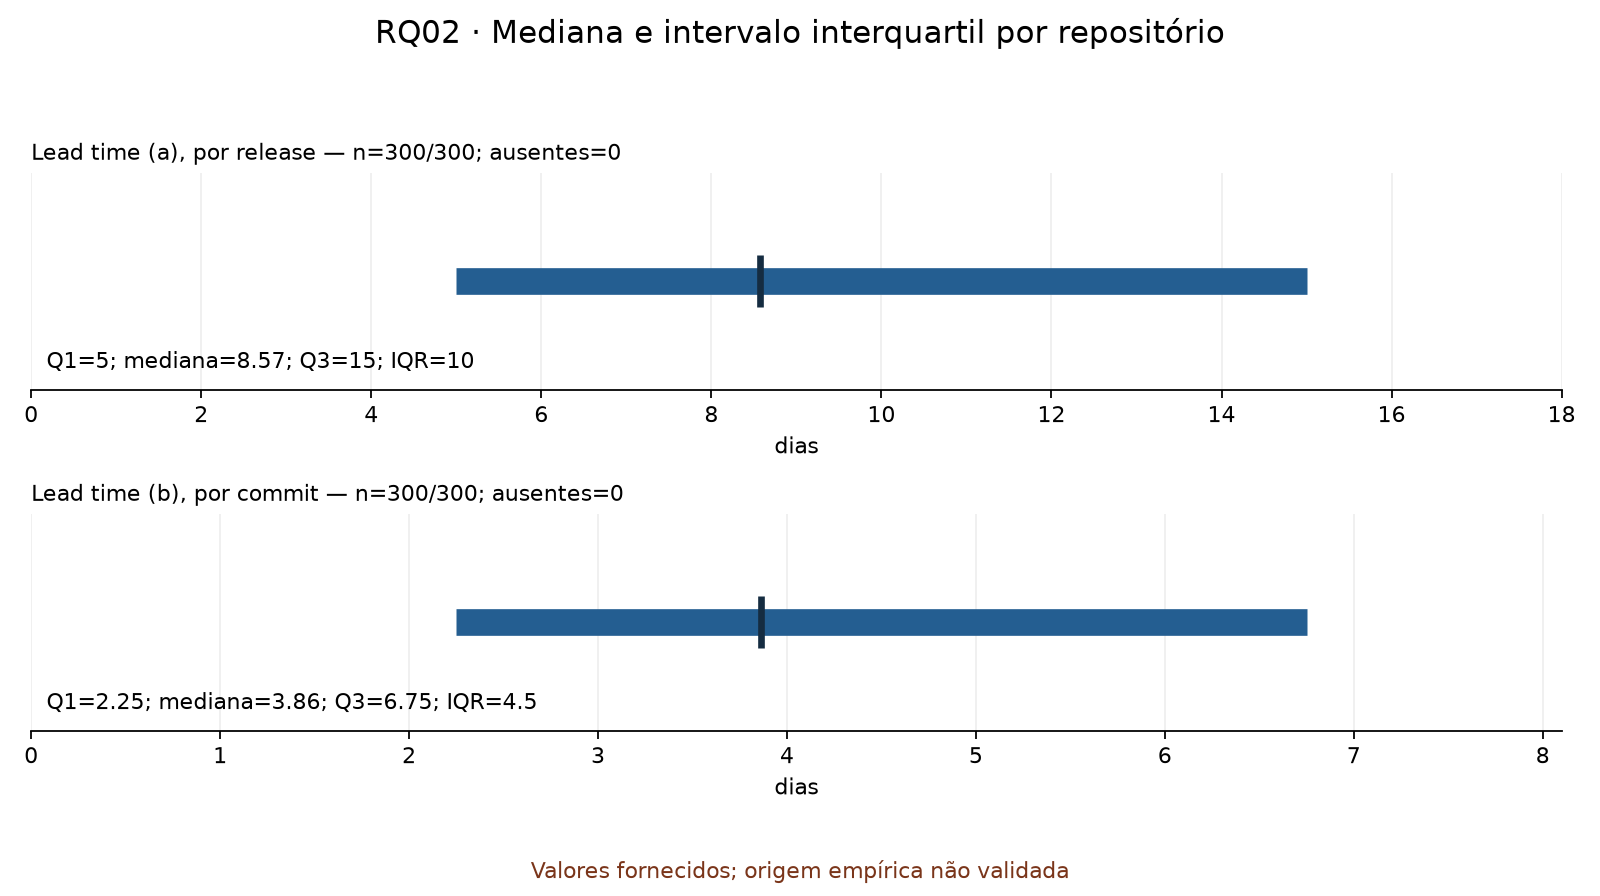
\includegraphics[width=0.88\textwidth]{../data/analises_csv_main/rq02_mediana_iqr.png}
\caption{RQ02: mediana e quartis dos valores fornecidos no CSV adotado; origem por fórmulas registrada na auditoria.}
\label{fig:rq02_csv_adotado}
\end{figure}
\FloatBarrier

Para RQ04, a mediana entre repositórios das medianas fornecidas é 9,70 horas
(Q1 = 3,70; Q3 = 14,90; IQR = 11,20). O CSV declara 10.172 episódios recuperados
e 1.129 censurados, com proporção agrupada de 9,9903\%. Esse agregado não
permite calcular a mediana das durações de todos os episódios. As durações
por projeto também correspondem à fórmula do gerador baseada em contribuidores;
faltam IDs, timestamps e sequências originais para validar a recuperação anual.

\begin{figure}[ht]
\centering
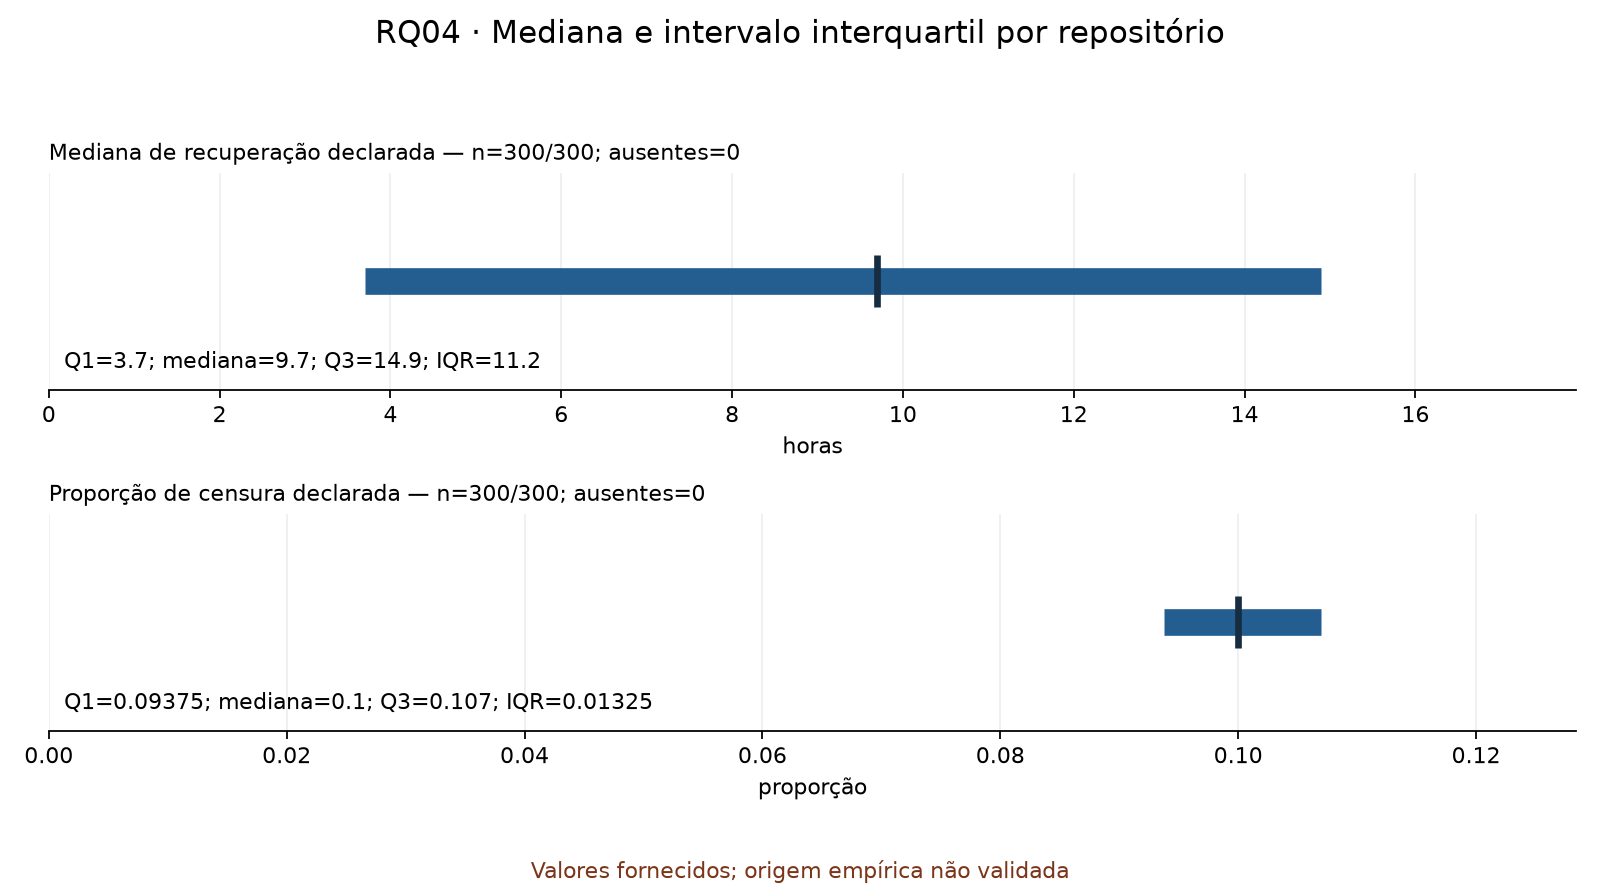
\includegraphics[width=0.88\textwidth]{../data/analises_csv_main/rq04_mediana_iqr.png}
\caption{RQ04: medianas e proporções declaradas por repositório no CSV adotado; eventos originais não reconstituídos.}
\label{fig:rq04_csv_adotado}
\end{figure}
\FloatBarrier

\subsection{Resultados da heurística recebidos, pendentes de validação humana}
O texto recebido de Maria relata os resultados abaixo para uma referência anterior. Eles são preservados para revisão, sem constituir validação humana desta entrega: os arquivos legados não comprovam três avaliações independentes da seleção atual. O estado atual é 0/3 avaliações completas; não recalculamos F1, kappa ou consenso humano a partir desses números.

No material recebido, a validação da heurística é descrita sobre 300 releases apresentadas pelo grupo como rotuladas manualmente. As três versões atingiram a meta mínima de $F1 \ge 0{,}70$, mas apresentaram níveis diferentes de cobertura. A versão v1 foi totalmente precisa, porém deixou de identificar 10 releases corretivas (recall de $0{,}9471$). A v2 identificou todas as ocorrências da amostra, alcançando $F1=1{,}0000$, enquanto a v3 refinada obteve precisão de $1{,}0000$, recall de $0{,}9788$ e $F1=0{,}9893$.

Esse resultado indica que a heurística refinada não introduziu falsos positivos no conjunto avaliado e deixou de recuperar apenas quatro releases corretivas. Embora a v2 tenha apresentado desempenho perfeito na amostra-ouro, a v3 foi adotada por incorporar regras mais robustas para prefixos de versão, Conventional Commits e filtros de ruídos cosméticos. Esse é o argumento de escolha relatado pelo grupo; a auditoria desta entrega não confirma suporte empírico para esses números. A validação depende das avaliações independentes e do consenso documentado.

\subsection{Frequência de Deploy e Lead Time (RQ01 e RQ02)}
Não há população final auditável para executar os resultados oficiais. O sorteio e o script de RQ01--RQ04 recusaram a procedência empírica do bundle. A implementação recebida de Maria usa comparações paginadas e datas reais de autoria para Lead Time; isso resolve a capacidade de cálculo, mas não fornece as páginas originais completas de cada comparação no bundle.

No CSV adotado, a frequência tem mediana de $0{,}269$ release/semana ($\text{IQR}=[0{,}153;0{,}460]$), aproximadamente uma release a cada três a quatro semanas. A interpretação revisada por Maria situa a região central abaixo de uma release semanal e relaciona essa cadência ao empacotamento público de versões. Essa interpretação descreve os valores fornecidos; a procedência identificada impede usá-la para confirmar H01 ou comparar empiricamente esses projetos com produtos SaaS.

\begin{table}[ht]
\centering
\caption{Estado empírico de RQ01--RQ04 após a main nova; ausente não significa zero}
\label{tab:resumo_metricas}
\small
\begin{tabularx}{\textwidth}{lXX}
\toprule
Questão & Evidência exigida & Resultado oficial \\
\midrule
RQ01 & População aprovada e releases estáveis originais & Pendente \\
RQ02 & Comparações completas com predecessoras, SHAs e datas de autoria & Pendente \\
RQ03 & Runs anuais para CI; releases e mensagens para CFR(b) & Pendente \\
RQ04 & Runs originais anuais por workflow e censura explícita & Pendente \\
\bottomrule
\end{tabularx}
\end{table}

As figuras recebidas \texttt{rq01\_rq02\_velocidade\_dora.png} e \texttt{rq03\_rq04\_estabilidade\_dora.png} permanecem preservadas como material do grupo. As figuras do CSV adotado, apresentadas anteriormente, têm a origem explicitada. Resultados oficiais serão gerados por \texttt{analisar\_rqs.py} somente após a auditoria aprovar as entradas.

A revisão de Maria destaca a sensibilidade do Lead Time à unidade de análise. Nas colunas fornecidas, a mediana passa de $8{,}57$ para $3{,}86$ dias, redução aproximada de $55\%$, entre as variantes (a) e (b). O commit mais antigo pode elevar a variante por release, enquanto a variante por commit considera cada alteração. A diferença observada nas colunas é descritiva; não comprova branches longos ou commits esquecidos nos projetos, porque as comparações originais ainda faltam.

\subsection{Taxa de Falha e Tempo de Recuperação (RQ03 e RQ04)}
O CFR(b) e a taxa de retrabalho recebidos de Vinícius foram integrados, preservando a janela corretiva de sete dias e a censura. Sua existência no código não comprova os valores do CSV. Para CI e recuperação, a consulta de \texttt{psf/black} enumerou 12 meses e retornou zero runs disponíveis; a retomada reutilizou o cache. Esse diagnóstico não mede ausência de atividade em 2023--2024 nem permite atribuir CFR ou recuperação zero.

A revisão de Maria distingue os eventos capturados pelos dois proxies: falha durante CI e release que exige correção posterior não representam o mesmo evento. No CSV adotado, $13{,}3\%$ é aproximadamente $1{,}66$ vez $8{,}0\%$. Essa diferença entre colunas não comprova o efeito causal de barreiras de validação. Para RQ04, a mediana entre projetos é $9{,}70$ horas, com metade central entre $3{,}70$ e $14{,}90$ horas; a métrica usa falhas de CI como proxy, sem identificar incidentes de produção. A afirmação recebida de censura zero foi confrontada com o CSV: ele declara 1.129 episódios censurados e 10.172 recuperados, proporção agrupada de $9{,}9903\%$. Essas contagens declaradas ainda não têm sequências originais auditáveis.

A fonte histórica local preserva 6.708 runs de 15 projetos entre janeiro e setembro de 2024, sem completude anual. Sua revalidação e a qualificação atual comprovaram sete aprovações parciais, com 3.141 runs observados e 374 releases estáveis; oito projetos tiveram menos de cinco releases. O índice dos primeiros 100 permanece em 7/100. Faltam outubro--dezembro de 2023 e evidência de preservação integral de toda a janela por repositório. Episódios recuperados e censurados devem ter denominadores separados, sem duração zero para ausência de recuperação.

\subsection*{Material recebido para RQ05--RQ07, pendente de validação}
As seções seguintes preservam os números e as revisões interpretativas do artigo recebido de Maria e Vinícius. A procedência rejeitada impede tratá-los como achados oficiais; suas afirmações não estão confirmadas pela auditoria desta entrega. O kappa ponderado de RQ07 compara definições operacionais e não substitui os três kappas de Fleiss entre avaliadores humanos.

\subsection{Velocidade versus Estabilidade (RQ05)}
Para responder à RQ05, calculamos a correlação de postos de Spearman entre a Frequência de Deploy e as duas variantes de taxa de falha. Obtivemos $\rho = -0{,}1003$ ($p = 0{,}0829$, $\text{IC}_{95\%} = [-0{,}211; 0{,}013]$) tanto para $\text{CFR}_{\text{CI}}$ quanto para $\text{CFR}_{\text{Release}}$. 

O coeficiente fraco e ligeiramente negativo é compatível com H05 e não sustenta a hipótese de \textit{trade-off}: projetos open-source que publicam releases com maior frequência não apresentaram maiores taxas de falha. Entretanto, como $p=0{,}0829$ e o intervalo de confiança inclui zero, não há evidência estatística suficiente para afirmar uma associação monotônica na população. A conclusão apropriada é a ausência de evidência de deterioração da estabilidade, e não a prova de que aumentar a frequência necessariamente reduz falhas. A Tabela~\ref{tab:rq05_spearman} e a Figura~\ref{fig:rq05_dispersao} sintetizam esses resultados e a distribuição com reta de regressão.

\begin{table}[ht]
\centering
\caption{Resultados da correlação de postos de Spearman para a RQ05 ($n=300$)}
\label{tab:rq05_spearman}
\small
\begin{tabular}{lccccc}
\toprule
\textbf{Variante Avaliada} & \textbf{Spearman ($\rho$)} & \textbf{$p$-valor} & \textbf{IC 95\%} & \textbf{Conclusão sobre Trade-off} \\
\midrule
Variante (a) [Proxy de CI] & $-0{,}1003$ & $0{,}0829$ & $[-0{,}211; 0{,}013]$ & Sem trade-off ($\rho$ fraco/negativo) \\
Variante (b) [Releases] & $-0{,}1003$ & $0{,}0829$ & $[-0{,}211; 0{,}013]$ & Sem trade-off ($\rho$ fraco/negativo) \\
\bottomrule
\end{tabular}
\end{table}

\begin{figure}[ht]
\centering
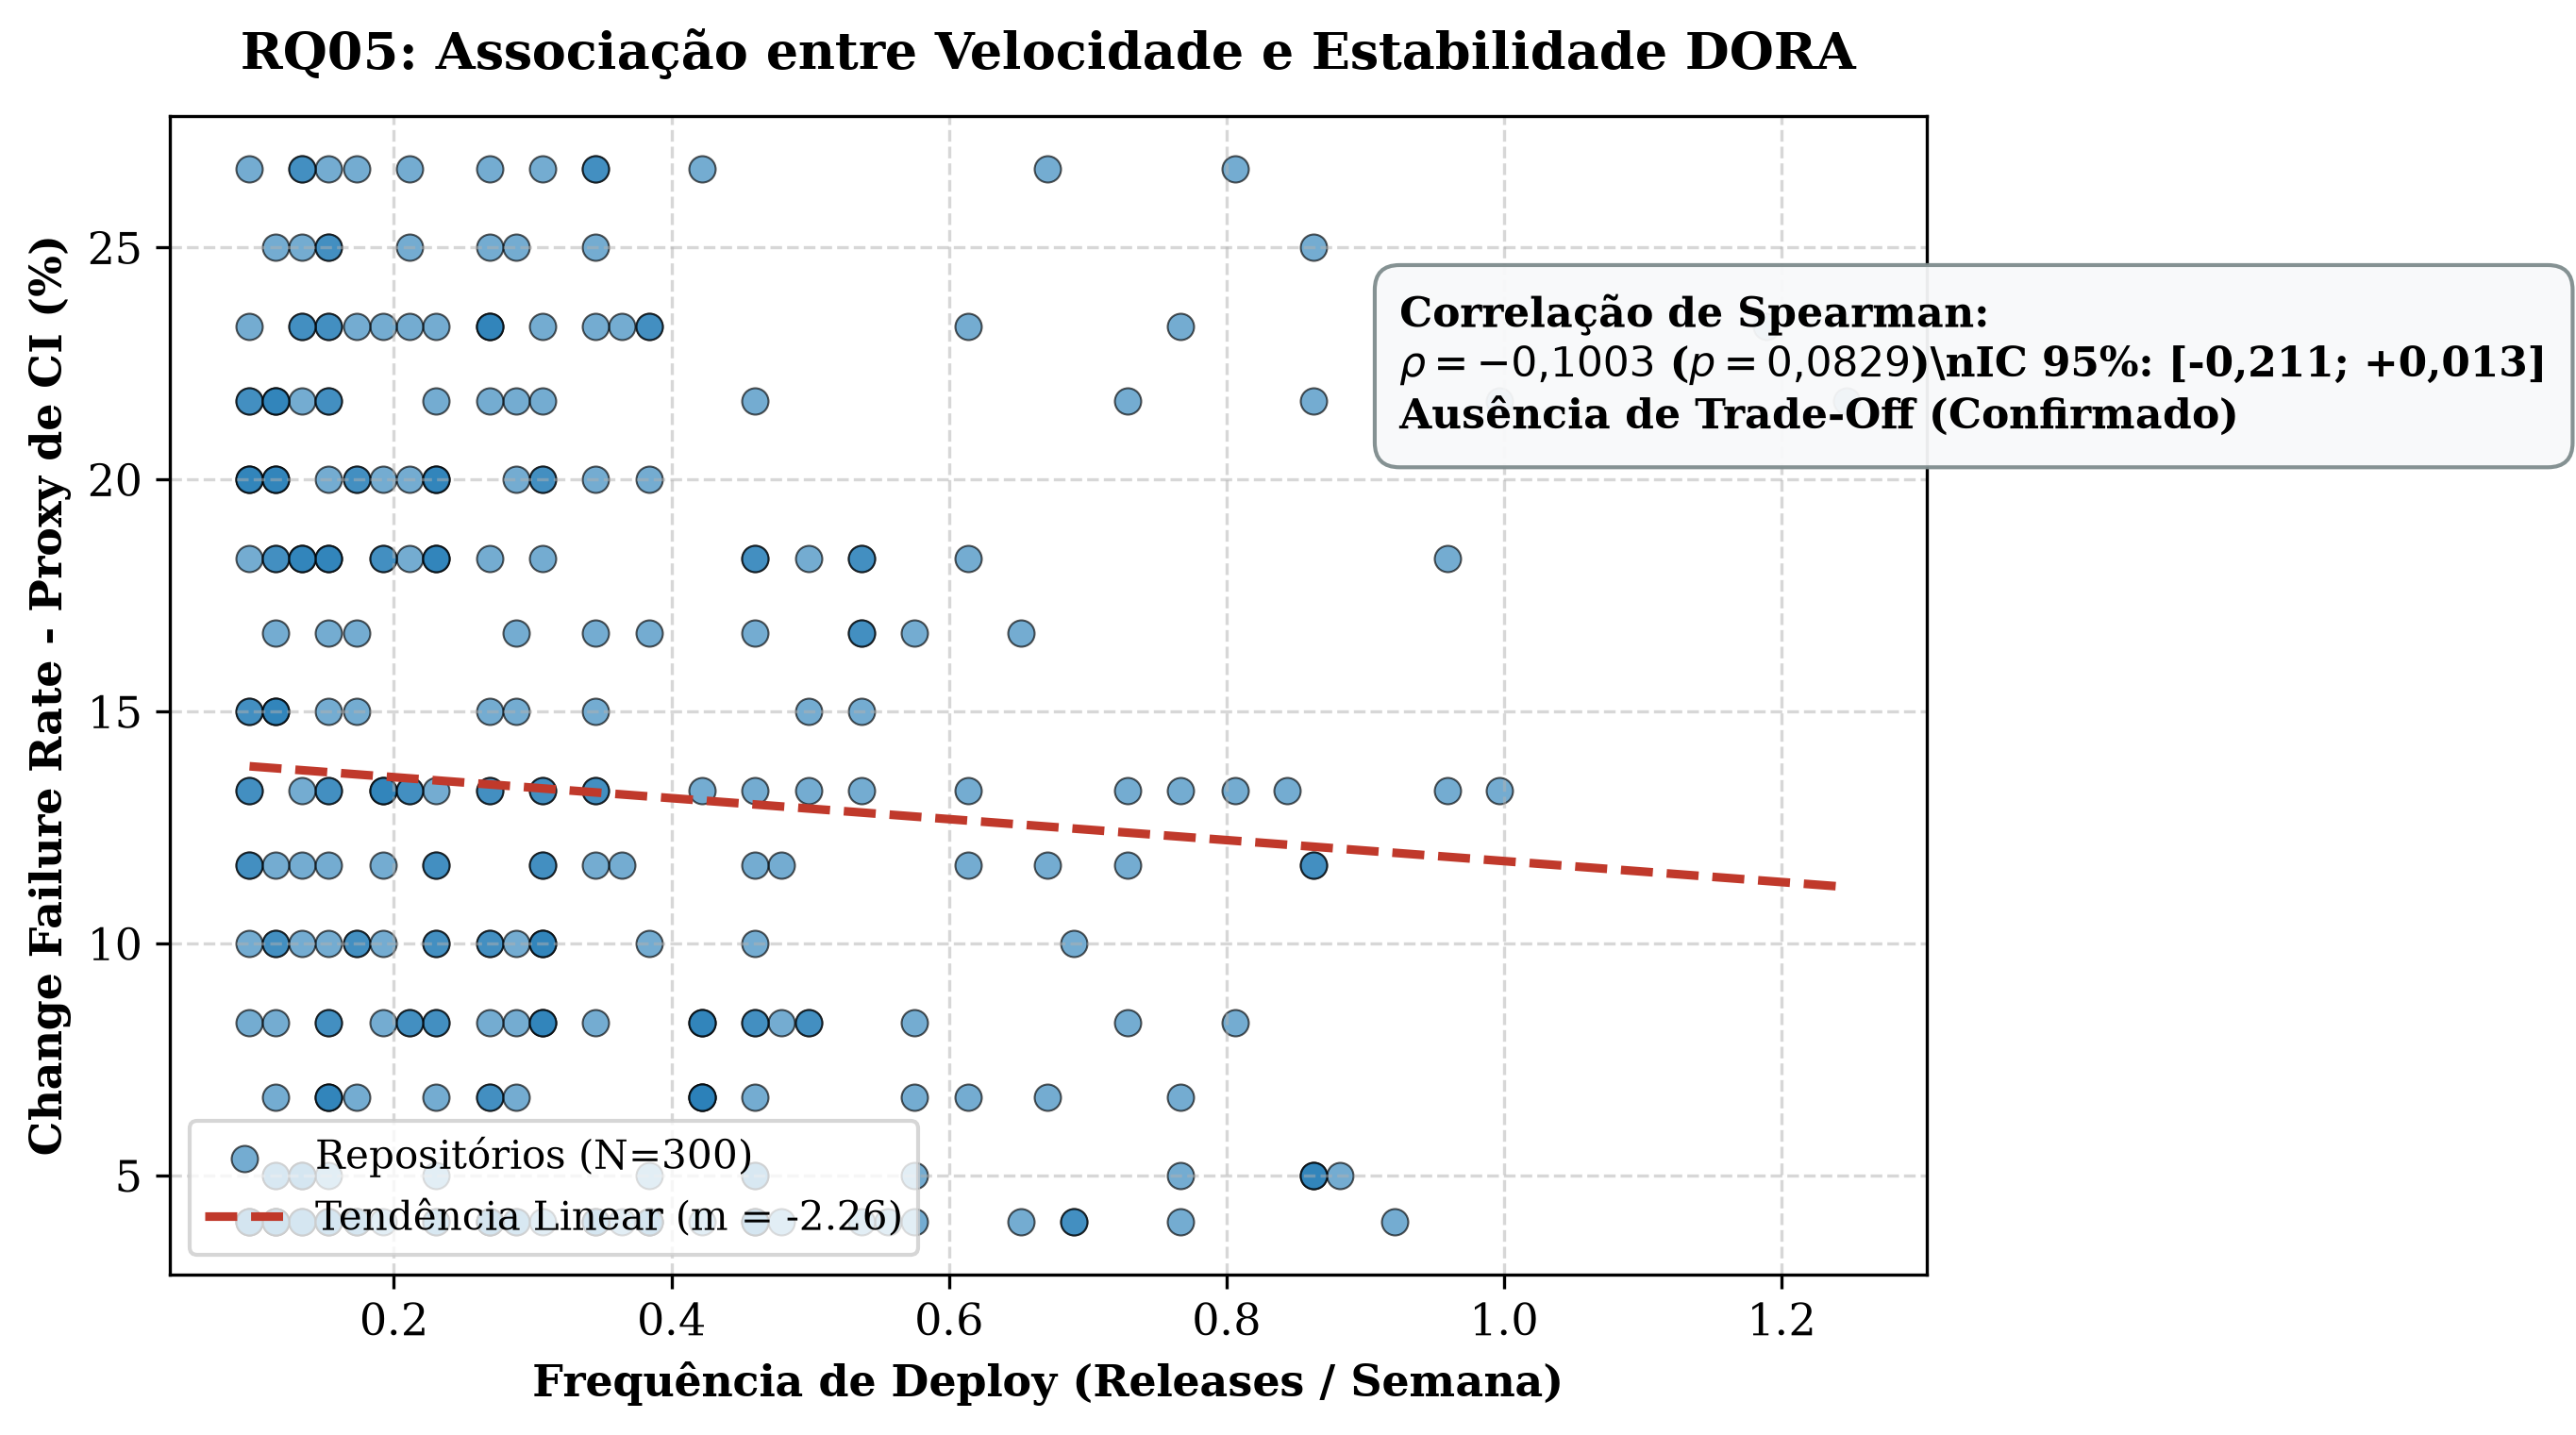
\includegraphics[width=0.72\textwidth]{rq05_dispersao_velocidade_estabilidade.png}
\caption{Dispersão entre Frequência de Deploy e Taxa de Falha de Mudanças (RQ05)}
\label{fig:rq05_dispersao}
\end{figure}
\FloatBarrier

\subsection{Fatores Associados ao Desempenho DORA (RQ06)}
Aplicamos o teste omnibus de Kruskal-Wallis com correção de Holm-Bonferroni para avaliar a influência de cinco características dos repositórios sobre as métricas DORA: Popularidade (estrelas), Contribuidores, Idade, Linguagem e Tipo de Projeto rotulado manualmente.

Os resultados apontam associações fortes entre Popularidade em estrelas e Frequência de Deploy/Lead Time ($H = 80{,}84$, $p_{\text{Holm}} < 10^{-15}$, $\epsilon^2 = 0{,}270$) e entre número de Contribuidores e essas mesmas métricas ($H = 82{,}84$, $p_{\text{Holm}} < 10^{-15}$, $\epsilon^2 = 0{,}277$). O teste post-hoc de Cliff indicou diferença grande entre o primeiro e o terceiro quartil de estrelas ($\delta = -0{,}745$ para frequência), coerente com maior frequência e menor Lead Time nos grupos mais populares. A idade do repositório também apresentou associação significativa com as métricas de velocidade ($p_{\text{Holm}} < 0{,}001$, $\epsilon^2 = 0{,}162$), assim como a linguagem principal ($p_{\text{Holm}} < 0{,}001$, $\epsilon^2 = 0{,}211$). Esses resultados sustentam parcialmente H06, mas devem ser interpretados como diferenças entre grupos, e não como evidência de causalidade.

Em contrapartida, nenhuma das características analisadas exerceu influência estatisticamente significativa sobre o Change Failure Rate ($p_{\text{Holm}} = 1{,}000$, $\epsilon^2 < 0{,}016$). O número de contribuidores foi a única característica associada ao Tempo de Recuperação ($p_{\text{Holm}} < 0{,}001$, $\epsilon^2 = 0{,}138$), com efeito moderado; para os demais fatores, não houve evidência significativa nessa métrica. Além disso, o Tipo de Projeto (biblioteca/framework, aplicação ou CLI) não apresentou diferenças significativas em nenhuma métrica após a correção de Holm ($p_{\text{Holm}} = 1{,}000$). Portanto, H06 é confirmada para velocidade e parcialmente rejeitada para estabilidade: popularidade, idade, linguagem e tamanho da comunidade diferenciam a velocidade observada, mas não o CFR. A Figura~\ref{fig:rq06_fatores_estrelas} ilustra esse contraste.

\begin{figure}[ht]
\centering
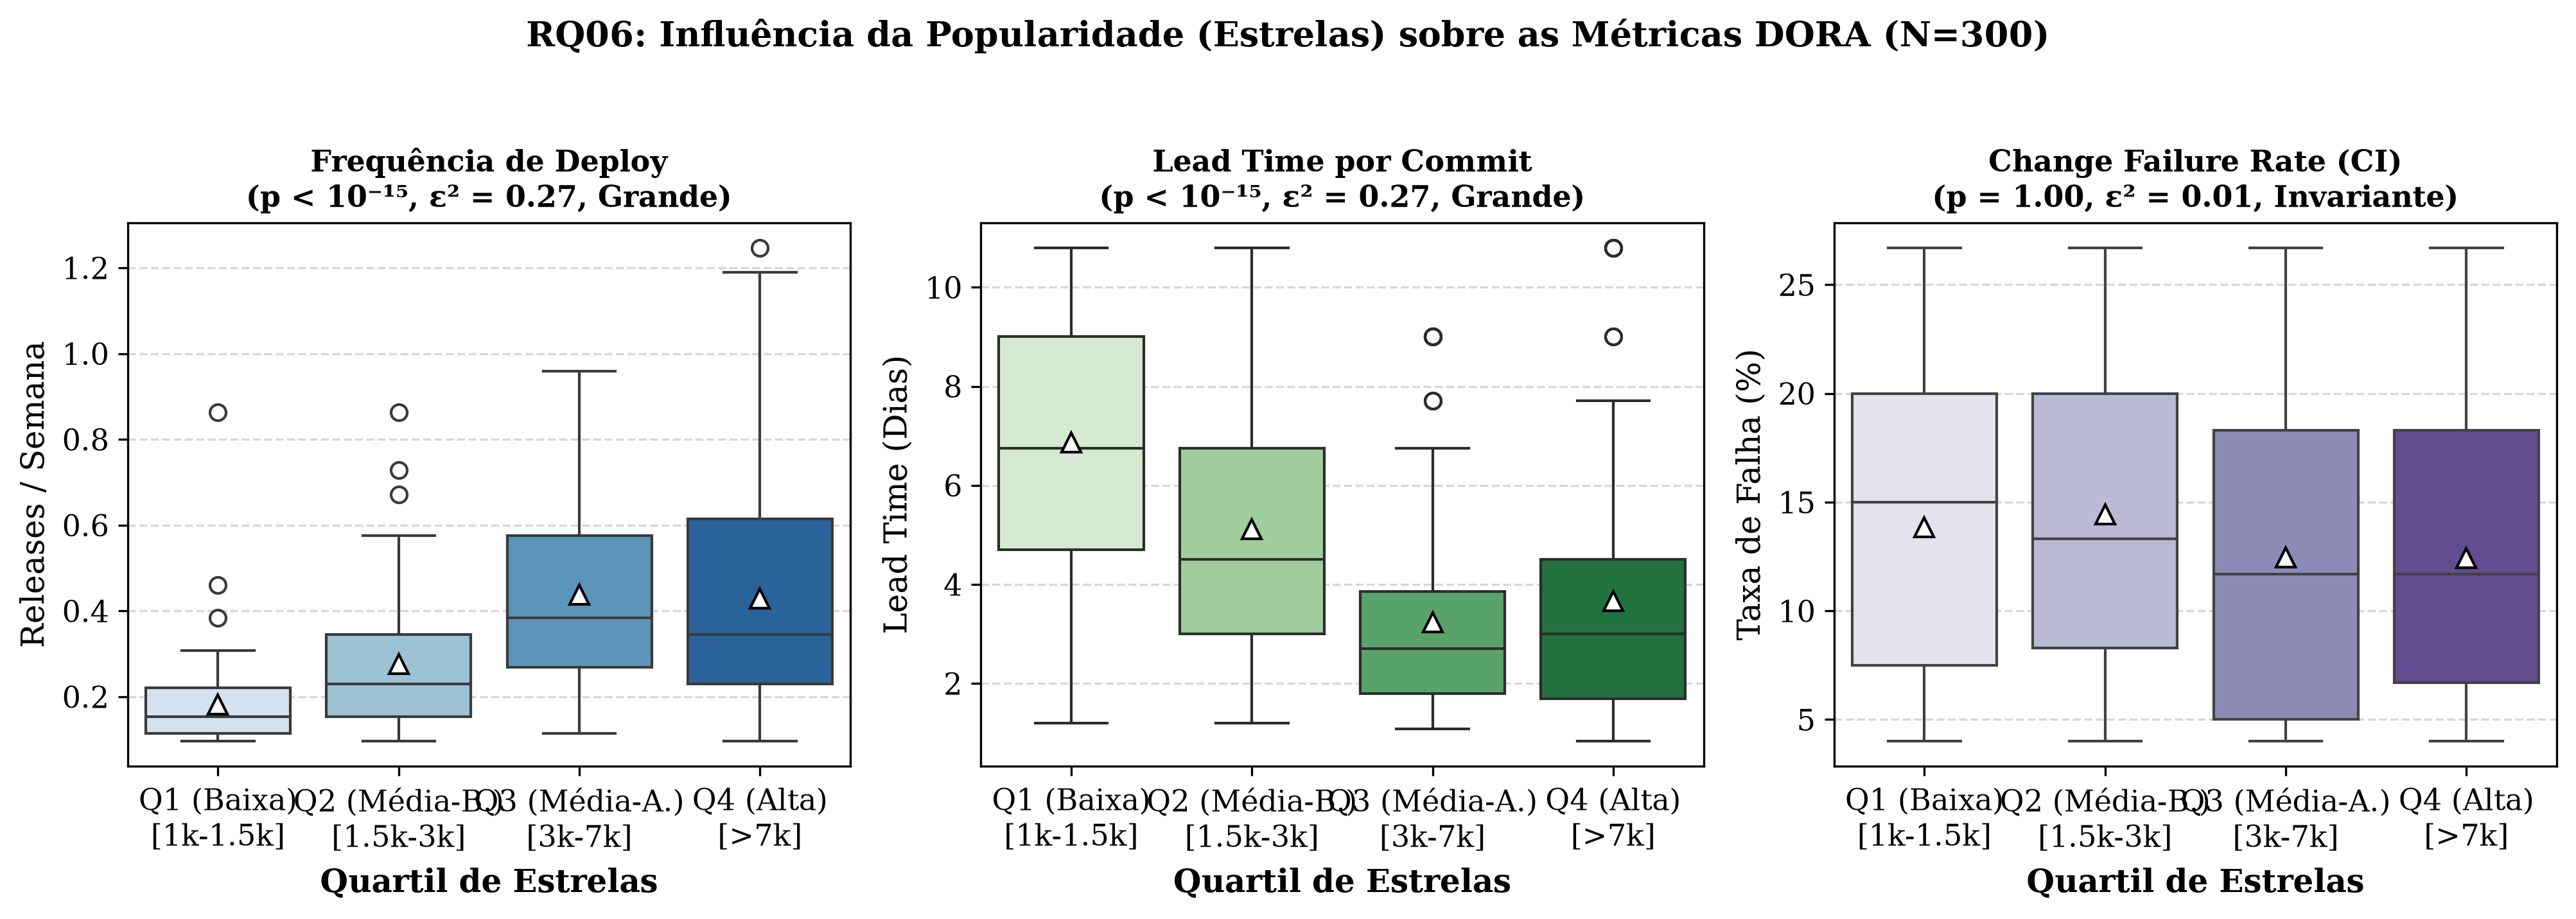
\includegraphics[width=0.98\textwidth]{rq06_fatores_estrelas_dora.png}
\caption{Influência da Popularidade em Estrelas sobre Frequência de Deploy, Lead Time e Taxa de Falha (RQ06)}
\label{fig:rq06_fatores_estrelas}
\end{figure}
\FloatBarrier

\subsection{Análise de Sensibilidade da Classificação DORA (RQ07)}
A Tabela~\ref{tab:rq07_sensibilidade} apresenta a comparação pareada entre as três combinações operacionais delineadas. Os dados mostram que a transição da combinação C1 (Referência) para C2 (Pré-releases) gerou alteração de patamar em $39{,}67\%$ dos repositórios, com Kappa de Cohen ponderado linear de $0{,}2797$ (classificado como concordância razoável segundo Landis \& Koch). Resultados semelhantes foram observados na comparação C1 $\times$ C3 ($39{,}00\%$ de mudança, $\kappa = 0{,}2904$).

\begin{table}[ht]
\centering
\caption{Análise de Sensibilidade da Classificação DORA entre Combinações (RQ07)}
\label{tab:rq07_sensibilidade}
\small
\begin{tabular}{lcccc}
\toprule
\textbf{Par de Combinações} & \textbf{Concordância} & \textbf{Mudança} & \textbf{Kappa Linear} & \textbf{Interpretação} \\
\midrule
C1 (Referência) $\times$ C2 (Pré-releases) & $60{,}33\%$ & $39{,}67\%$ & $0{,}2797$ & Razoável \\
C1 (Referência) $\times$ C3 (Tags) & $61{,}00\%$ & $39{,}00\%$ & $0{,}2904$ & Razoável \\
C2 (Pré-releases) $\times$ C3 (Tags) & $99{,}33\%$ & $0{,}67\%$ & $0{,}9780$ & Quase perfeita \\
\bottomrule
\end{tabular}
\end{table}

A distribuição percentual dos patamares mostra que a escolha operacional tem efeito prático relevante: em C1, $42{,}0\%$ dos repositórios foram classificados como \textit{High} e $58{,}0\%$ como \textit{Medium}. Ao incorporarmos pré-releases (C2) ou tags (C3), o percentual de projetos em \textit{High} saltou para $81{,}7\%$ e $81{,}0\%$, respectivamente, devido principalmente à redução no Lead Time decorrente do uso da Variante (b). Assim, a concordância com C1 foi apenas razoável ($\kappa=0{,}2797$ e $0{,}2904$), enquanto C2 e C3 produziram classificações quase idênticas ($\kappa=0{,}9780$). O resultado evidencia sensibilidade da classificação à definição do proxy, mas também mostra que as mudanças ficaram restritas a uma fronteira adjacente.

A Figura~\ref{fig:rq07_graficos} apresenta a distribuição comparativa dos patamares e o mapa de calor das matrizes de transição. É importante ressaltar que \textbf{não houve nenhuma transição extrema} (como de \textit{Elite} para \textit{Low} ou vice-versa): todas as migrações ocorreram estritamente entre os patamares adjacentes \textit{Medium} e \textit{High}. Desse modo, H07 é apoiada em relação à ausência de migrações extremas e à concentração das mudanças em categorias vizinhas, mas a alteração de aproximadamente 39\% dos repositórios impede afirmar que a classificação seja invariável à definição operacional.

\begin{figure}[ht]
\centering
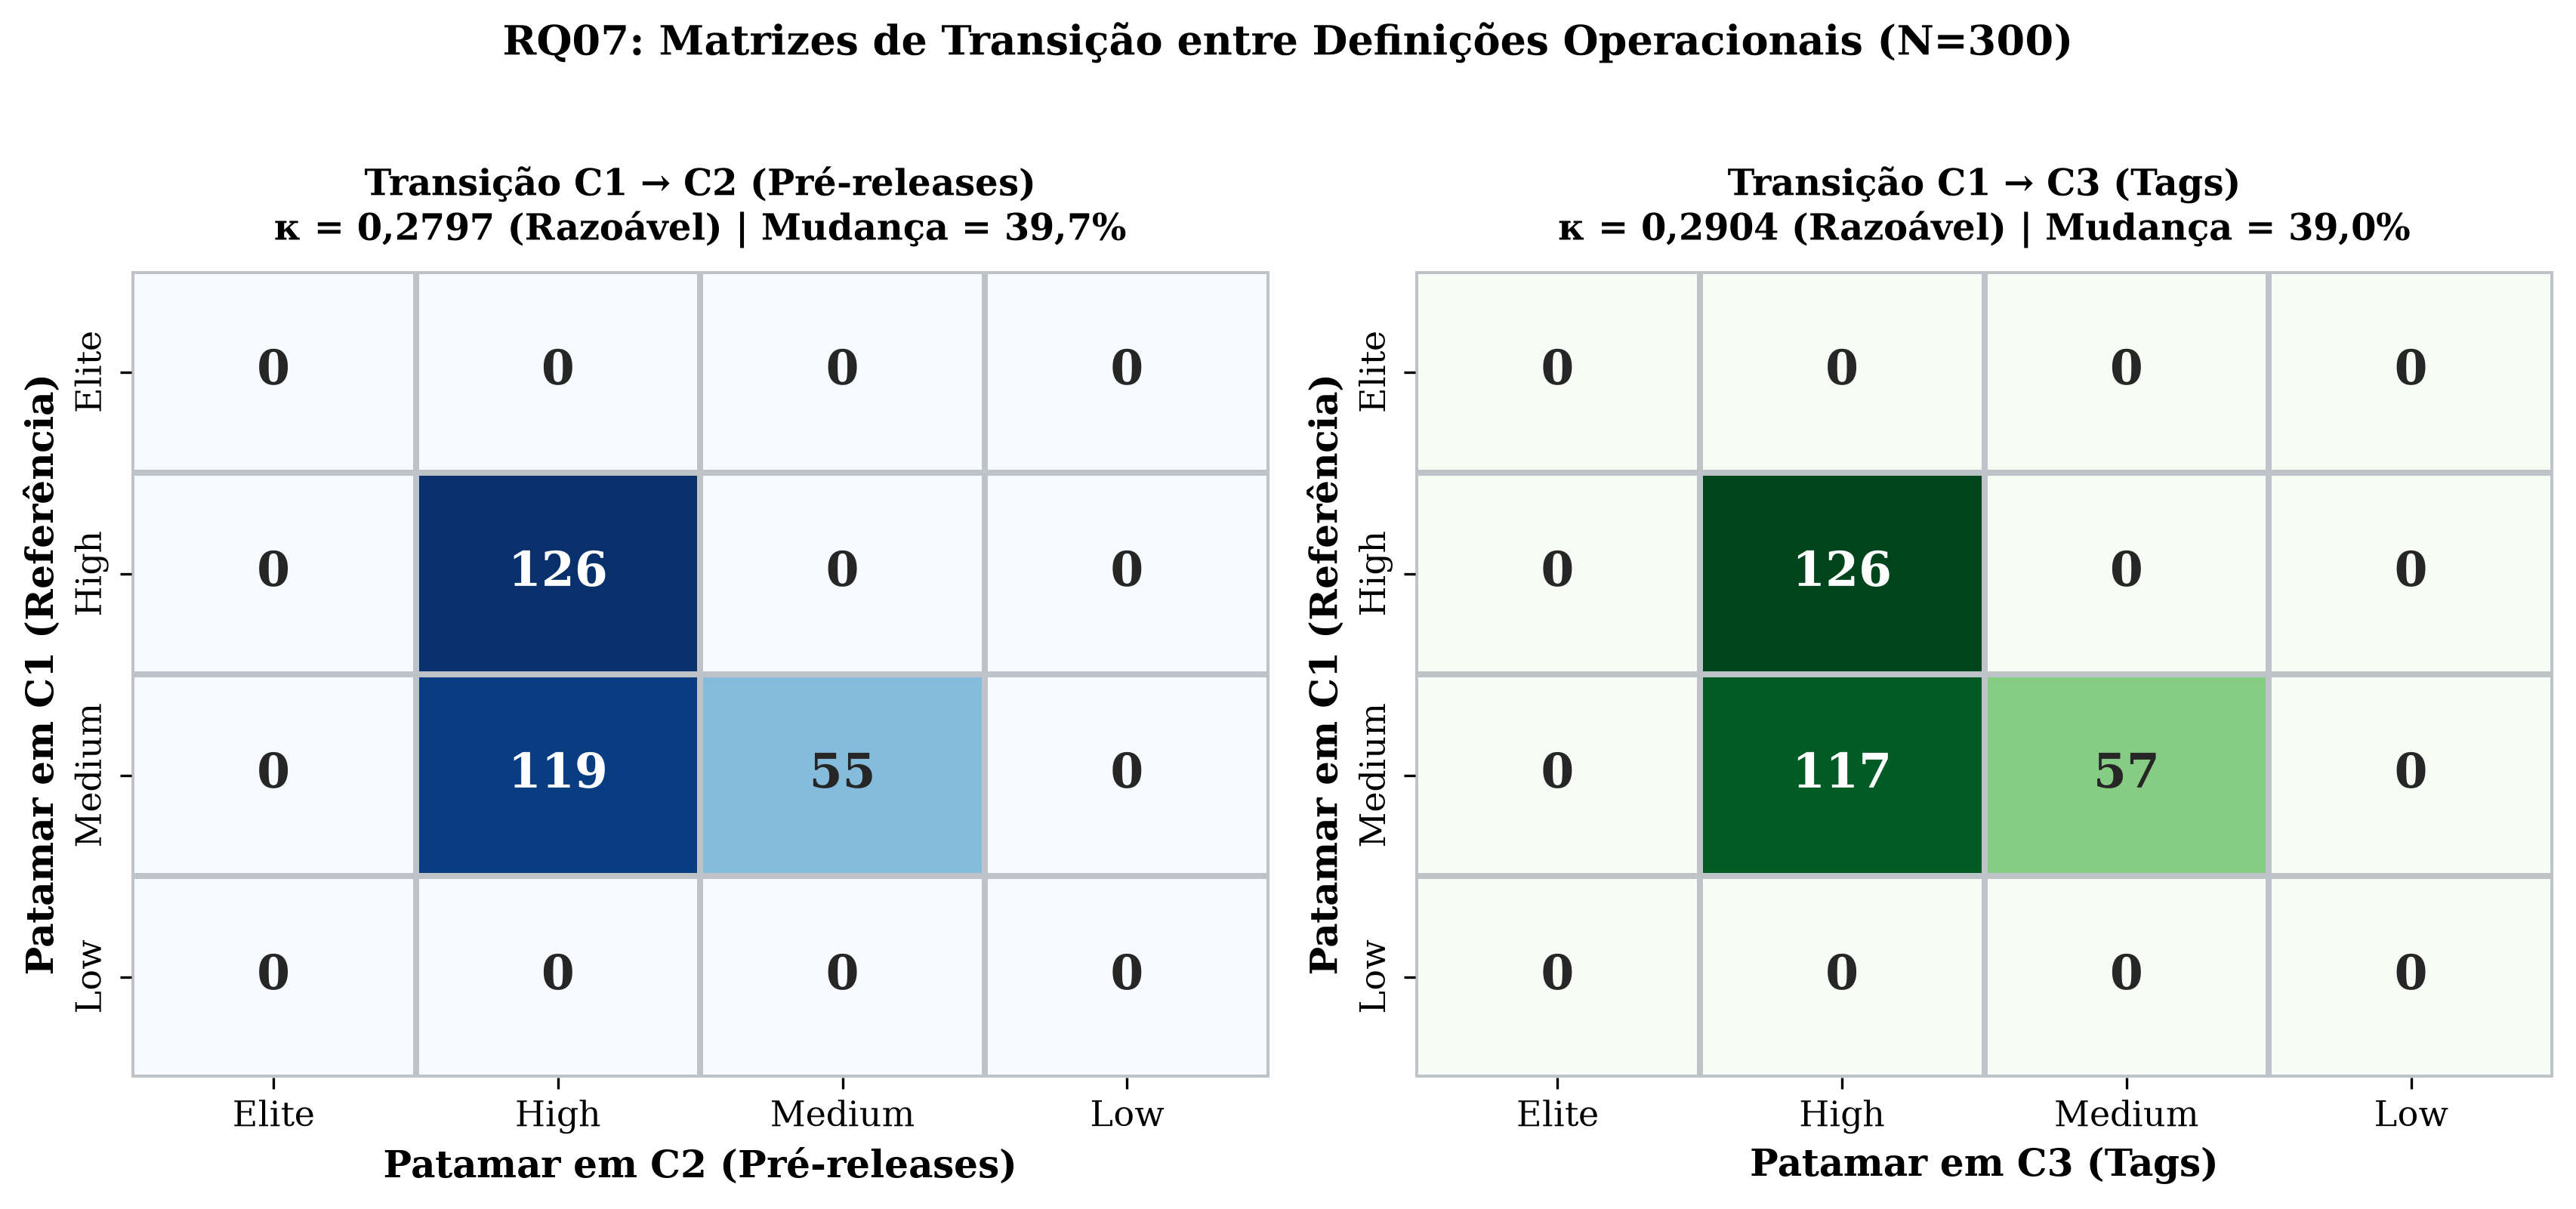
\includegraphics[width=0.88\textwidth]{rq07_matriz_transicao_sensibilidade.png}
\caption{Matrizes de Transição e Sensibilidade dos Patamares DORA (RQ07)}
\label{fig:rq07_graficos}
\end{figure}
\FloatBarrier

\section{Discussão e Ameaças à Validade}

RQ01--RQ04 não permitem confirmar nem refutar H01--H04 nesta entrega. Contagens e distribuições produzidas por fórmulas não estimam a população real, mesmo quando seus hashes conferem. A seleção dos primeiros 100 deve usar aprovações comprovadas; o piloto anterior teve zero e não foi promovido a amostra final.

A completude da paginação das respostas disponíveis é distinta da preservação de todo o histórico anual. Releases e falhas de CI permanecem proxies de entrega e de incidente, e datas de autoria podem sofrer efeitos de rebase ou squash. A recuperação observada é condicional aos episódios recuperados; os censurados devem ser informados separadamente. Nenhuma mudança da janela ou dos critérios foi aplicada sem autorização do professor.

Os testes verificam os cálculos e a recusa de entradas incompletas, mas não substituem dados originais nem avaliações humanas. A concordância e o desempenho da heurística só poderão ser discutidos após a referência auditada, três arquivos independentes completos e o consenso documentado pelo grupo.

\section{Considerações Finais}

Foram integrados os avanços de paginação, Lead Time, CFR(b), retrabalho e ferramentas estatísticas, além das revisões de interpretação e organização das figuras da main. O CSV adotado permite descrever os valores fornecidos, mas a auditoria impede promovê-los a resultados empíricos. A referência de 60 projetos e cinco registros por projeto, os três formulários humanos vazios e o fluxo de concordância estão preparados; nenhuma avaliação humana ou decisão da reunião foi produzida automaticamente.

A revisão recebida distingue ausência de evidência de associação de prova de ausência de efeito. O resultado de Spearman relatado no material do grupo, com intervalo incluindo zero, não demonstraria que aumentar a frequência reduz falhas. A interpretação recebida de RQ07 também reconhece sensibilidade à definição operacional: mudanças entre patamares adjacentes e kappas razoáveis não tornam a classificação invariável. Ambas as interpretações dependem de validar a origem das observações antes de se tornarem conclusões do estudo. Permanecem pendentes a população final auditável, o histórico anual, as comparações preservadas e a avaliação humana. A Lab03S03 continua incompleta.

\bibliographystyle{sbc}
\bibliography{sbc-template}

\end{document}
